% Koma class
\documentclass[a4paper, oneside]{scrartcl}   

\usepackage{a4wide}

%------------------
% language = english
\usepackage[english, german]{babel}	% Umlaute mit \"u
\usepackage[latin1]{inputenc}

% margins + Kopf- und Fu�zeilen
\usepackage[left = 2.5cm, right = 2.5cm, top = 2cm, bottom = 3cm]{geometry}
\usepackage{scrpage2} 
\pagestyle{scrheadings}
\clearscrheadfoot
\rehead{\headmark}
\lehead{\pagemark}
\lohead{\headmark}
\rohead{\pagemark} 


% math
\usepackage{amssymb}
\usepackage{amsmath}

% figures
\usepackage{tikz}
\usepackage{graphicx}


% section-Zaehler wird neu gesetzt:
\setcounter{section}{7}
%------------------
\author{Sascha Meiers, Martin Seeger}
\title{Exercise 7, Discrete Mathematics for Bioinformatics}
\date{Winter term 2011/2012}


\begin{document}
\maketitle

%---------------------------------------------------------------------------------------------------

\subsection{Network Flow (Niveau II)}

\begin{description}
\item[a) $\Rightarrow$ b)] This is the same as the Theorem on pp. 5006-5007
in the lecture since the existence of an augmenting path is equivalent to
the reachability of $t$ from $s$ in the residual network $G_f$. If there is such
a path then $f$ is not a maximum.
\item[b) $\Rightarrow$ c)] Assume there is no augmenting path in $G_f$ from $s$
to $t$. Let 
\[
S = \{ v \in V | \exists\  \mathrm{path}\  s \leadsto t\  \mathrm{in}\  G_f\},
\ T = V \backslash S.
\]
Then $(S, T)$ is a cut because $s \in S$ and $T \notin S$. \\
It is easy to see that this cut is saturated by $f$: pick $(u, v) \in S\times
T$. If $(u, v) \in E$, hence $(u, v) \in E \cap S\times
T$ then if $f(u, v) < \mathrm{cap}(u, v)$, $v$ would become reachable from $u$
and hence also from $s$. Therefore $f(u, v) = \mathrm{cap}(u, v)$.
On the other hand, assume $(v, u) \in E$, i.e. $(u, v) \in E \cap T\times
S$. Then if $f(u, v) > 0$, we would have $v \in S$ which means that really $f(u,
v) = 0$. Therefore $f$ saturates $(S, T)$. By the Lemma on p. 5006, $\mathrm{val}(f) =
\mathrm{cap}(S, T)$.
\item[c) $\Rightarrow$ a)] We have by the Lemma on p. 5006 that for any flow $f$
and cut $(S, T)$
\[
\mathrm{val}(f) \leq  \mathrm{cap}(S, T).
\]
Therefore a flow which saturates this inequality must be maximal.
\end{description}
In summary, we have given an construction for a minimum cut that satisfies the
Max-Flow Min-Cut Theorem given a maximum flow resp. its residual network.

\subsection{Network Flow (Niveau I)}
Replace each node $v$ with its associated \emph{node capacity} $c_v$ by two new nodes 
$v_{in}, v_{out}$ and an edge $(v_{in},v_{out})$ with \emph{edge capacity} $c_v$. Then all ingoing 
edges $(u,v) \in E$ point to $v_{in}$, the outgoing edges $(v,u) \in E$ start from $v_{out}$.   


\subsection{Ford-Fulkerson}

The first figure shows the residual network according to the current flow. 
An augmenting path is marked in green.

The Ford-Fulkerson algorithm uses this path to increase the network flow by 1. 
After that the residual network as seen on the right remains. There is no augmenting path left, 
as a breadth-first search can decide. The same breadth-first search (see green arrow) 
is used to find a minimum cut (see red line), which has a capacity of 10.

\begin{minipage}[hb]{\textwidth}
\begin{center}
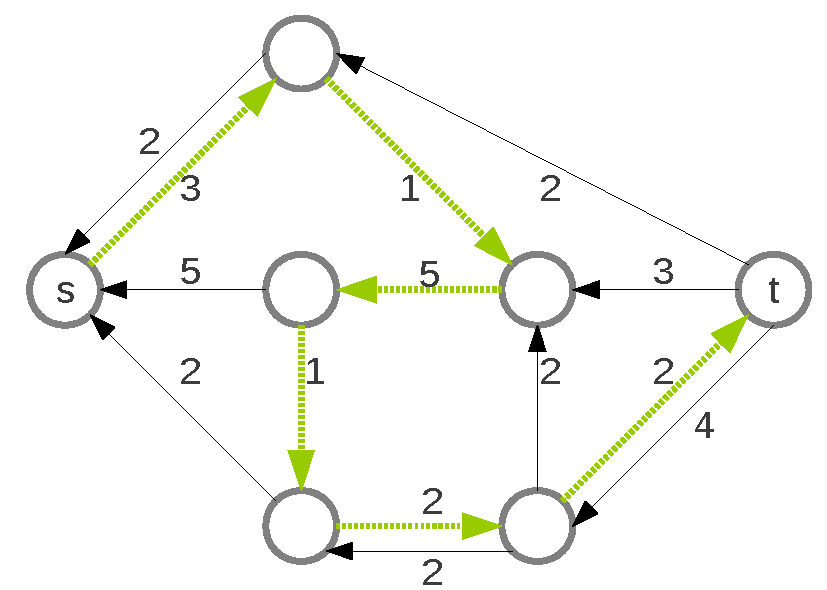
\includegraphics[width=7cm]{restnetz1.pdf}
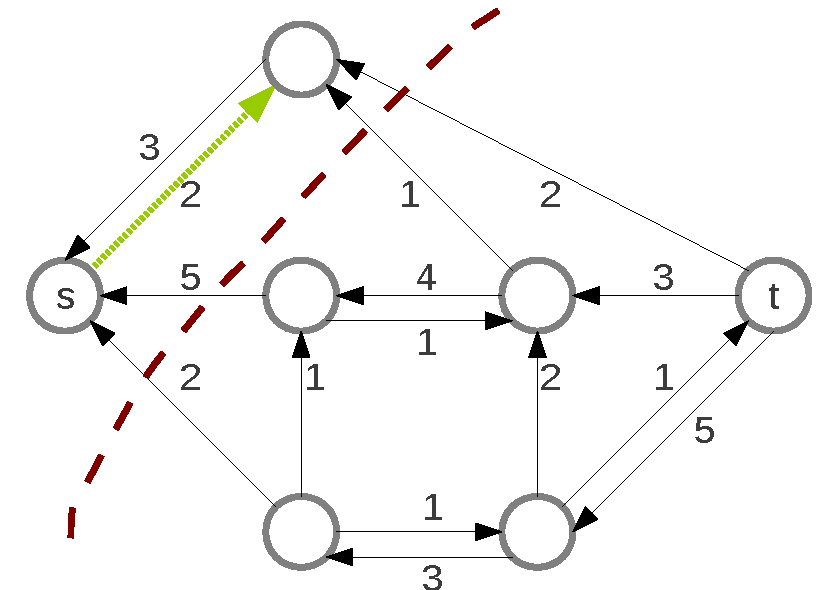
\includegraphics[width=7cm]{restnetz2.pdf}
\end{center}
\end{minipage}


\subsection{Bipartite matching}

The figure below shows the augmenting-path method to find a optimal matching in a bipartite graph.
The set of edges concerned for the matching are marked black and in each step we label a remaining 
augemting path in blue.
\begin{center}
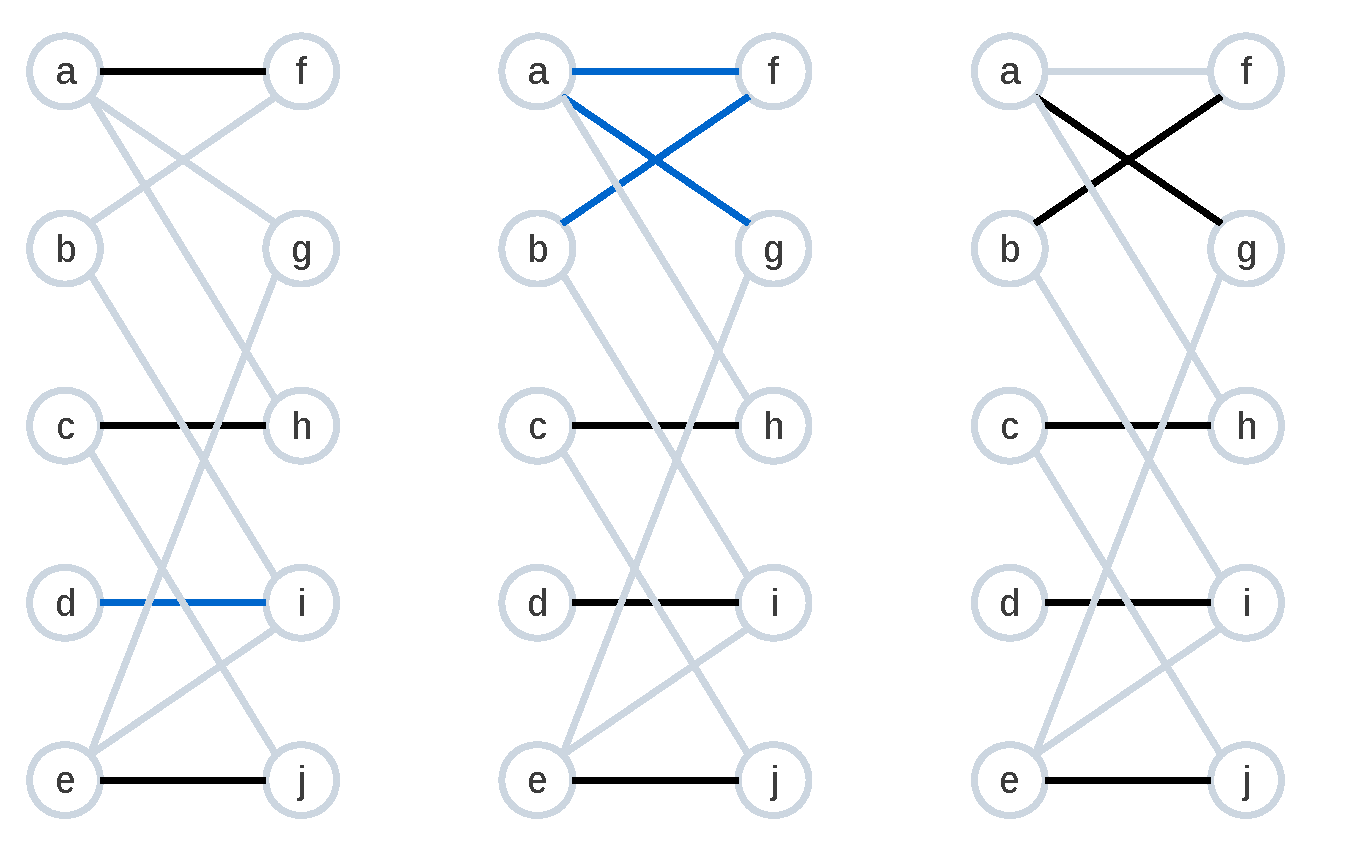
\includegraphics[width=12cm]{bipartite_matching.pdf}
\end{center}









\end{document}
